\section{Implementation of the FVM in 1D}
The code to solve the SWE in 1D using FVM is based on the Godunov scheme with the exact Riemann solver.
The exact solution of the Riemann problem is found by using the Riemann invariants and the Rankine-Hugoniot conditions~\cite{trento_course}.

The true solution is found by solving the Riemann problem exact, with 5000 cells, and distinguishing between the wetbed or drybed case, and also identifying the shock and rarefaction waves.


\section{Godunov's Method}
We consider the Godunov Upwind method, which is a first-order accurate metod to solve non-linear systems of hyperbolic conservation laws~\cite{Toro2024}.
Godunov's method is a fundamental starting point.
In the method we solve the non-linear Riemann problem at each cell interface. 

Consider the initial-boundary value problem (IBVP) for a system of $N$ nonlinear hyperbolic conservation (balance?) laws     
\begin{equation}\label{eq:IBVP_system}
    \begin{cases}
    \text{PDEs: }    &\mathbf{U}_t + \mathbf{F(U)}_x = \mathbf{S(U)}, \quad x \in [a, b], \quad t > 0, \\
    \text{ICs: }    &\mathbf{U}(x,0) = \mathbf{U}^{(0)}(x), \quad x \in [a,b], \\
    \text{BCs: }    &\mathbf{U}(a,t) = \mathbf{B}_{L}(t), \quad \mathbf{U}(b,t) = \mathbf{B}_{R}(t), \quad t \geq 0.
    \end{cases}
\end{equation}
The vectors $\mathbf{B}_L (t)$ and $\mathbf{B}_R (t)$ denote the boundary conditions at the left and right boundaries, respectively.
The Godunov Upwind method in conservative form~\eqref{eq:explicit_conservative_1D_SWE} solves the IBVP~\eqref{eq:IBVP_system}.


\section{Data generation}
The data generation is done by solving the SWE in 1D using the FVM with the Godunov scheme and the exact Riemann solver.
We use Gaussian functions with parametric extension~\cite{Gaussian} to generate the initial conditions, that is, functions on the form
\begin{align*}
    h(x,0) &= a \exp{\left(\frac{-{(x-\mu)}^2}{2\sigma^2}\right)}, \\
\end{align*}
where $a$ is the amplitude of the Gaussian, $\mu$ is the mean value, and $\sigma$ is the standard deviation.
We solve the 1D SWE with the following parameters:
\begin{itemize}
    \item $N = 200$ cells,
    \item From $t = 0.0$ to $t_{\text{end}} = 1.0$,
    \item $x \in [0, 1]$,
    \item $u(x,0) = 0$,
    \item $b(x) = 0.0$,
    \item $g = 9.81$ and
    \item $\sigma = 0.1$.
\end{itemize}
The value of $\mu$ is varied to generate different initial conditions, as seen in Figure~\ref{fig:data_generation_initial}.
\begin{figure}[H]
    \centering
    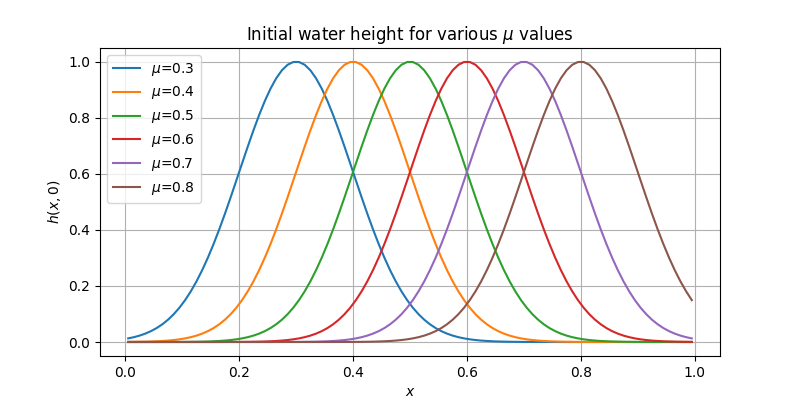
\includegraphics[width=0.8\textwidth]{C:/Users/Matteo/Shallow-Water-Equations/plots/data_generation_initial.png}
    \caption{Initial conditions for the data generation.}\label{fig:data_generation_initial}
\end{figure}



